\subsection{UC3 - Riduzione dimensionale}
\begin{figure}[h]
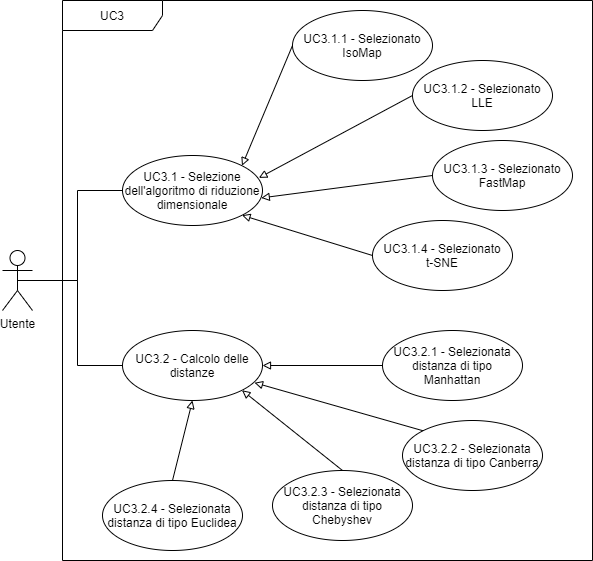
\includegraphics[width=14cm]{section/Images/UC3.png}
\centering
\caption{UC3 - Riduzione dimensionale}
\end{figure}
\begin{itemize}
	\item \textbf{Attore primario}: Utente;
	\item \textbf{Precondizioni}: L'utente ha caricato i dati e le dimensioni nel sistema [UC1];
	\item \textbf{Postcondizioni}: Le nuove dimensioni vengono inserite nel sistema e sono disponibili all'utente per la visualizzazione [UC5];
	\item \textbf{Scenario principale}: L'utente può creare nuove dimensioni, a partire da quelle caricate [UC1] ed eventualmente scremate [UC2] o prodotte da iterazioni precedenti, tramite:
	\begin{enumerate}[1.]
		\item Algoritmo di riduzione dimensionale [UC3.1];
		\item Calcolo delle distanze tra i valori delle dimensioni [UC3.2].
	\end{enumerate}
	L'utente potrà selezionare le dimensioni interessate dalla riduzione tramite apposite celle per poi premere il tasto di conferma; le nuove dimensioni saranno visualizzate insieme alle precedenti per, eventualmente, procedere in modo iterativo.
\end{itemize}